\documentclass[1p]{elsarticle_modified}
%\bibliographystyle{elsarticle-num}

%\usepackage[colorlinks]{hyperref}
%\usepackage{abbrmath_seonhwa} %\Abb, \Ascr, \Acal ,\Abf, \Afrak
\usepackage{amsfonts}
\usepackage{amssymb}
\usepackage{amsmath}
\usepackage{amsthm}
\usepackage{scalefnt}
\usepackage{amsbsy}
\usepackage{kotex}
\usepackage{caption}
\usepackage{subfig}
\usepackage{color}
\usepackage{graphicx}
\usepackage{xcolor} %% white, black, red, green, blue, cyan, magenta, yellow
\usepackage{float}
\usepackage{setspace}
\usepackage{hyperref}

\usepackage{tikz}
\usetikzlibrary{arrows}

\usepackage{multirow}
\usepackage{array} % fixed length table
\usepackage{hhline}

%%%%%%%%%%%%%%%%%%%%%
\makeatletter
\renewcommand*\env@matrix[1][\arraystretch]{%
	\edef\arraystretch{#1}%
	\hskip -\arraycolsep
	\let\@ifnextchar\new@ifnextchar
	\array{*\c@MaxMatrixCols c}}
\makeatother %https://tex.stackexchange.com/questions/14071/how-can-i-increase-the-line-spacing-in-a-matrix
%%%%%%%%%%%%%%%

\usepackage[normalem]{ulem}

\newcommand{\msout}[1]{\ifmmode\text{\sout{\ensuremath{#1}}}\else\sout{#1}\fi}
%SOURCE: \msout is \stkout macro in https://tex.stackexchange.com/questions/20609/strikeout-in-math-mode

\newcommand{\cancel}[1]{
	\ifmmode
	{\color{red}\msout{#1}}
	\else
	{\color{red}\sout{#1}}
	\fi
}

\newcommand{\add}[1]{
	{\color{blue}\uwave{#1}}
}

\newcommand{\replace}[2]{
	\ifmmode
	{\color{red}\msout{#1}}{\color{blue}\uwave{#2}}
	\else
	{\color{red}\sout{#1}}{\color{blue}\uwave{#2}}
	\fi
}

\newcommand{\Sol}{\mathcal{S}} %segment
\newcommand{\D}{D} %diagram
\newcommand{\A}{\mathcal{A}} %arc


%%%%%%%%%%%%%%%%%%%%%%%%%%%%%5 test

\def\sl{\operatorname{\textup{SL}}(2,\Cbb)}
\def\psl{\operatorname{\textup{PSL}}(2,\Cbb)}
\def\quan{\mkern 1mu \triangleright \mkern 1mu}

\theoremstyle{definition}
\newtheorem{thm}{Theorem}[section]
\newtheorem{prop}[thm]{Proposition}
\newtheorem{lem}[thm]{Lemma}
\newtheorem{ques}[thm]{Question}
\newtheorem{cor}[thm]{Corollary}
\newtheorem{defn}[thm]{Definition}
\newtheorem{exam}[thm]{Example}
\newtheorem{rmk}[thm]{Remark}
\newtheorem{alg}[thm]{Algorithm}

\newcommand{\I}{\sqrt{-1}}
\begin{document}

%\begin{frontmatter}
%
%\title{Boundary parabolic representations of knots up to 8 crossings}
%
%%% Group authors per affiliation:
%\author{Yunhi Cho} 
%\address{Department of Mathematics, University of Seoul, Seoul, Korea}
%\ead{yhcho@uos.ac.kr}
%
%
%\author{Seonhwa Kim} %\fnref{s_kim}}
%\address{Center for Geometry and Physics, Institute for Basic Science, Pohang, 37673, Korea}
%\ead{ryeona17@ibs.re.kr}
%
%\author{Hyuk Kim}
%\address{Department of Mathematical Sciences, Seoul National University, Seoul 08826, Korea}
%\ead{hyukkim@snu.ac.kr}
%
%\author{Seokbeom Yoon}
%\address{Department of Mathematical Sciences, Seoul National University, Seoul, 08826,  Korea}
%\ead{sbyoon15@snu.ac.kr}
%
%\begin{abstract}
%We find all boundary parabolic representation of knots up to 8 crossings.
%
%\end{abstract}
%\begin{keyword}
%    \MSC[2010] 57M25 
%\end{keyword}
%
%\end{frontmatter}

%\linenumbers
%\tableofcontents
%
\newcommand\colored[1]{\textcolor{white}{\rule[-0.35ex]{0.8em}{1.4ex}}\kern-0.8em\color{red} #1}%
%\newcommand\colored[1]{\textcolor{white}{ #1}\kern-2.17ex	\textcolor{white}{ #1}\kern-1.81ex	\textcolor{white}{ #1}\kern-2.15ex\color{red}#1	}

{\Large $\underline{12n_{0829}~(K12n_{0829})}$}

\setlength{\tabcolsep}{10pt}
\renewcommand{\arraystretch}{1.6}
\vspace{1cm}\begin{tabular}{m{100pt}>{\centering\arraybackslash}m{274pt}}
\multirow{5}{120pt}{
	\centering
	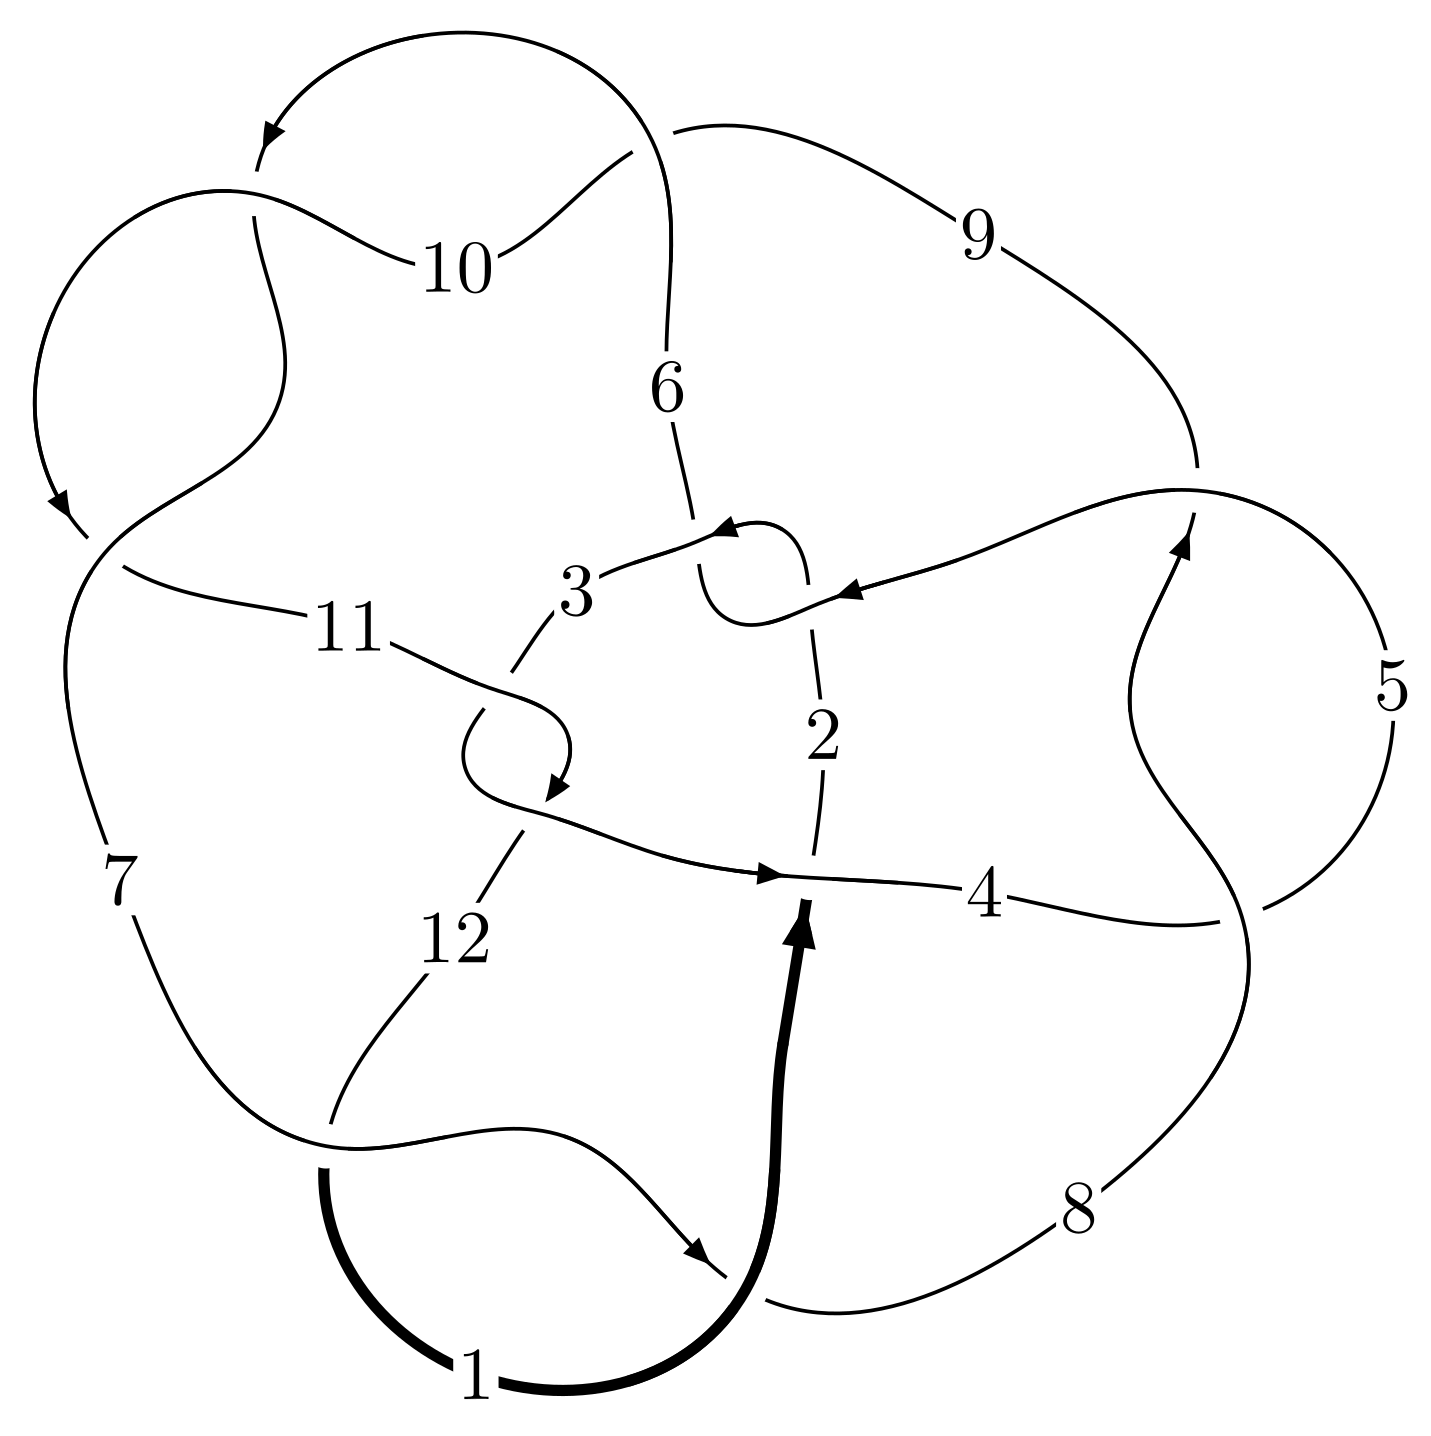
\includegraphics[width=112pt]{../../../GIT/diagram.site/Diagrams/png/2918_12n_0829.png}\\
\ \ \ A knot diagram\footnotemark}&
\allowdisplaybreaks
\textbf{Linearized knot diagam} \\
\cline{2-2}
 &
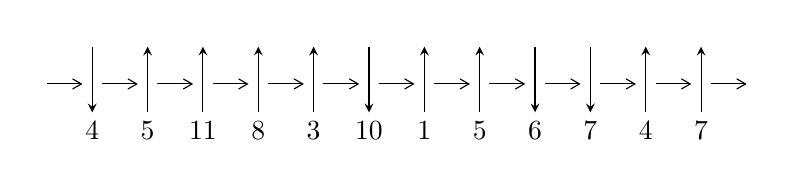
\begin{tikzpicture}[x=20pt, y=17pt]
	% nodes
	\node (C0) at (0, 0) {};
	\node (C1) at (1, 0) {};
	\node (C1U) at (1, +1) {};
	\node (C1D) at (1, -1) {4};

	\node (C2) at (2, 0) {};
	\node (C2U) at (2, +1) {};
	\node (C2D) at (2, -1) {5};

	\node (C3) at (3, 0) {};
	\node (C3U) at (3, +1) {};
	\node (C3D) at (3, -1) {11};

	\node (C4) at (4, 0) {};
	\node (C4U) at (4, +1) {};
	\node (C4D) at (4, -1) {8};

	\node (C5) at (5, 0) {};
	\node (C5U) at (5, +1) {};
	\node (C5D) at (5, -1) {3};

	\node (C6) at (6, 0) {};
	\node (C6U) at (6, +1) {};
	\node (C6D) at (6, -1) {10};

	\node (C7) at (7, 0) {};
	\node (C7U) at (7, +1) {};
	\node (C7D) at (7, -1) {1};

	\node (C8) at (8, 0) {};
	\node (C8U) at (8, +1) {};
	\node (C8D) at (8, -1) {5};

	\node (C9) at (9, 0) {};
	\node (C9U) at (9, +1) {};
	\node (C9D) at (9, -1) {6};

	\node (C10) at (10, 0) {};
	\node (C10U) at (10, +1) {};
	\node (C10D) at (10, -1) {7};

	\node (C11) at (11, 0) {};
	\node (C11U) at (11, +1) {};
	\node (C11D) at (11, -1) {4};

	\node (C12) at (12, 0) {};
	\node (C12U) at (12, +1) {};
	\node (C12D) at (12, -1) {7};
	\node (C13) at (13, 0) {};

	% arrows
	\draw[->,>={angle 60}]
	(C0) edge (C1) (C1) edge (C2) (C2) edge (C3) (C3) edge (C4) (C4) edge (C5) (C5) edge (C6) (C6) edge (C7) (C7) edge (C8) (C8) edge (C9) (C9) edge (C10) (C10) edge (C11) (C11) edge (C12) (C12) edge (C13) ;	\draw[->,>=stealth]
	(C1U) edge (C1D) (C2D) edge (C2U) (C3D) edge (C3U) (C4D) edge (C4U) (C5D) edge (C5U) (C6U) edge (C6D) (C7D) edge (C7U) (C8D) edge (C8U) (C9U) edge (C9D) (C10U) edge (C10D) (C11D) edge (C11U) (C12D) edge (C12U) ;
	\end{tikzpicture} \\
\hhline{~~} \\& 
\textbf{Solving Sequence} \\ \cline{2-2} 
 &
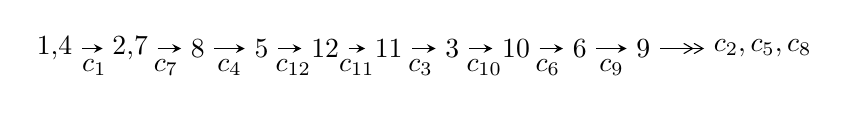
\begin{tikzpicture}[x=23pt, y=7pt]
	% node
	\node (A0) at (-1/8, 0) {1,4};
	\node (A1) at (17/16, 0) {2,7};
	\node (A2) at (17/8, 0) {8};
	\node (A3) at (25/8, 0) {5};
	\node (A4) at (33/8, 0) {12};
	\node (A5) at (41/8, 0) {11};
	\node (A6) at (49/8, 0) {3};
	\node (A7) at (57/8, 0) {10};
	\node (A8) at (65/8, 0) {6};
	\node (A9) at (73/8, 0) {9};
	\node (C1) at (1/2, -1) {$c_{1}$};
	\node (C2) at (13/8, -1) {$c_{7}$};
	\node (C3) at (21/8, -1) {$c_{4}$};
	\node (C4) at (29/8, -1) {$c_{12}$};
	\node (C5) at (37/8, -1) {$c_{11}$};
	\node (C6) at (45/8, -1) {$c_{3}$};
	\node (C7) at (53/8, -1) {$c_{10}$};
	\node (C8) at (61/8, -1) {$c_{6}$};
	\node (C9) at (69/8, -1) {$c_{9}$};
	\node (A10) at (11, 0) {$c_{2},c_{5},c_{8}$};

	% edge
	\draw[->,>=stealth]	
	(A0) edge (A1) (A1) edge (A2) (A2) edge (A3) (A3) edge (A4) (A4) edge (A5) (A5) edge (A6) (A6) edge (A7) (A7) edge (A8) (A8) edge (A9) ;
	\draw[->>,>={angle 60}]	
	(A9) edge (A10);
\end{tikzpicture} \\ 

\end{tabular} \\

\footnotetext{
The image of knot diagram is generated by the software ``\textbf{Draw programme}" developed by Andrew Bartholomew(\url{http://www.layer8.co.uk/maths/draw/index.htm\#Running-draw}), where we modified some parts for our purpose(\url{https://github.com/CATsTAILs/LinksPainter}).
}\phantom \\ \newline 
\centering \textbf{Ideals for irreducible components\footnotemark of $X_{\text{par}}$} 
 
\begin{align*}
I^u_{1}&=\langle 
-246065 u^{16}-4244217 u^{15}+\cdots+5347744 b-62370976,\\
\phantom{I^u_{1}}&\phantom{= \langle  }-1456963 u^{16}-16357645 u^{15}+\cdots+10695488 a-33380064,\;u^{17}+13 u^{16}+\cdots+384 u+64\rangle \\
I^u_{2}&=\langle 
32 u^{21} a+3841 u^{21}+\cdots+32 a+7087,\;-4960 u^{21} a-3211 u^{21}+\cdots-9433 a-7311,\\
\phantom{I^u_{2}}&\phantom{= \langle  }u^{22}-5 u^{21}+\cdots+9 u-1\rangle \\
I^u_{3}&=\langle 
-395 u^7+1362 u^6-2821 u^5+528 u^4+4313 u^3-6033 u^2+499 b+2843 u+219,\\
\phantom{I^u_{3}}&\phantom{= \langle  }176 u^7-881 u^6+2212 u^5-2254 u^4-1376 u^3+5528 u^2+499 a-5591 u+2405,\\
\phantom{I^u_{3}}&\phantom{= \langle  }u^8-4 u^7+9 u^6-5 u^5-11 u^4+22 u^3-15 u^2+u+1\rangle \\
I^u_{4}&=\langle 
u^3 a+2 u^2 a+u^3- a u+2 u^2+b+a+1,\;- u^2 a+2 u^3+a^2- a u+6 u^2+2 a+2 u-3,\;u^4+3 u^3+u^2- u+1\rangle \\
\\
\end{align*}
\raggedright * 4 irreducible components of $\dim_{\mathbb{C}}=0$, with total 77 representations.\\
\footnotetext{All coefficients of polynomials are rational numbers. But the coefficients are sometimes approximated in decimal forms when there is not enough margin.}
\newpage
\renewcommand{\arraystretch}{1}
\centering \section*{I. $I^u_{1}= \langle -2.46\times10^{5} u^{16}-4.24\times10^{6} u^{15}+\cdots+5.35\times10^{6} b-6.24\times10^{7},\;-1.46\times10^{6} u^{16}-1.64\times10^{7} u^{15}+\cdots+1.07\times10^{7} a-3.34\times10^{7},\;u^{17}+13 u^{16}+\cdots+384 u+64 \rangle$}
\flushleft \textbf{(i) Arc colorings}\\
\begin{tabular}{m{7pt} m{180pt} m{7pt} m{180pt} }
\flushright $a_{1}=$&$\begin{pmatrix}1\\0\end{pmatrix}$ \\
\flushright $a_{4}=$&$\begin{pmatrix}0\\u\end{pmatrix}$ \\
\flushright $a_{2}=$&$\begin{pmatrix}1\\u^2\end{pmatrix}$ \\
\flushright $a_{7}=$&$\begin{pmatrix}0.136222 u^{16}+1.52940 u^{15}+\cdots+24.6566 u+3.12095\\0.0460129 u^{16}+0.793646 u^{15}+\cdots+55.1943 u+11.6630\end{pmatrix}$ \\
\flushright $a_{8}=$&$\begin{pmatrix}0.182235 u^{16}+2.32304 u^{15}+\cdots+79.8509 u+14.7840\\0.0460129 u^{16}+0.793646 u^{15}+\cdots+55.1943 u+11.6630\end{pmatrix}$ \\
\flushright $a_{5}=$&$\begin{pmatrix}0.0357957 u^{16}+0.746991 u^{15}+\cdots+66.8882 u+12.8825\\-0.281648 u^{16}-3.00567 u^{15}+\cdots+1.86308 u+2.29092\end{pmatrix}$ \\
\flushright $a_{12}=$&$\begin{pmatrix}-0.317443 u^{16}-3.75266 u^{15}+\cdots-66.0251 u-9.59153\\0.281648 u^{16}+3.00567 u^{15}+\cdots-0.863078 u-2.29092\end{pmatrix}$ \\
\flushright $a_{11}=$&$\begin{pmatrix}-0.317443 u^{16}-3.75266 u^{15}+\cdots-66.0251 u-9.59153\\-0.00420439 u^{16}-0.702547 u^{15}+\cdots-124.203 u-26.2336\end{pmatrix}$ \\
\flushright $a_{3}=$&$\begin{pmatrix}-0.0865400 u^{16}-1.32604 u^{15}+\cdots-66.0553 u-12.4275\\0.486877 u^{16}+5.63364 u^{15}+\cdots+103.536 u+18.4041\end{pmatrix}$ \\
\flushright $a_{10}=$&$\begin{pmatrix}-0.199312 u^{16}-2.38217 u^{15}+\cdots-56.2845 u-9.51523\\0.201025 u^{16}+1.92542 u^{15}+\cdots-20.8039 u-5.53856\end{pmatrix}$ \\
\flushright $a_{6}=$&$\begin{pmatrix}-0.519547 u^{16}-5.47455 u^{15}+\cdots-26.4448 u-3.93239\\-0.869649 u^{16}-9.93344 u^{15}+\cdots-149.357 u-26.0336\end{pmatrix}$ \\
\flushright $a_{9}=$&$\begin{pmatrix}0.866357 u^{16}+10.0713 u^{15}+\cdots+194.012 u+35.2369\\0.995891 u^{16}+11.9801 u^{15}+\cdots+303.450 u+58.3917\end{pmatrix}$\\&\end{tabular}
\flushleft \textbf{(ii) Obstruction class $= -1$}\\~\\
\flushleft \textbf{(iii) Cusp Shapes $= \frac{2547627}{668468} u^{16}+\frac{7779965}{167117} u^{15}+\cdots+\frac{235542904}{167117} u+\frac{48416750}{167117}$}\\~\\
\newpage\renewcommand{\arraystretch}{1}
\flushleft \textbf{(iv) u-Polynomials at the component}\newline \\
\begin{tabular}{m{50pt}|m{274pt}}
Crossings & \hspace{64pt}u-Polynomials at each crossing \\
\hline $$\begin{aligned}c_{1}\end{aligned}$$&$\begin{aligned}
&u^{17}-13 u^{16}+\cdots+384 u-64
\end{aligned}$\\
\hline $$\begin{aligned}c_{2},c_{3},c_{5}\\c_{11}\end{aligned}$$&$\begin{aligned}
&u^{17}- u^{16}+\cdots+2 u^2-1
\end{aligned}$\\
\hline $$\begin{aligned}c_{4},c_{7},c_{8}\\c_{12}\end{aligned}$$&$\begin{aligned}
&u^{17}- u^{16}+\cdots+2 u-1
\end{aligned}$\\
\hline $$\begin{aligned}c_{6},c_{9},c_{10}\end{aligned}$$&$\begin{aligned}
&u^{17}+7 u^{16}+\cdots+20 u-8
\end{aligned}$\\
\hline
\end{tabular}\\~\\
\newpage\renewcommand{\arraystretch}{1}
\flushleft \textbf{(v) Riley Polynomials at the component}\newline \\
\begin{tabular}{m{50pt}|m{274pt}}
Crossings & \hspace{64pt}Riley Polynomials at each crossing \\
\hline $$\begin{aligned}c_{1}\end{aligned}$$&$\begin{aligned}
&y^{17}+y^{16}+\cdots+30720 y-4096
\end{aligned}$\\
\hline $$\begin{aligned}c_{2},c_{3},c_{5}\\c_{11}\end{aligned}$$&$\begin{aligned}
&y^{17}- y^{16}+\cdots+4 y-1
\end{aligned}$\\
\hline $$\begin{aligned}c_{4},c_{7},c_{8}\\c_{12}\end{aligned}$$&$\begin{aligned}
&y^{17}-7 y^{16}+\cdots+16 y-1
\end{aligned}$\\
\hline $$\begin{aligned}c_{6},c_{9},c_{10}\end{aligned}$$&$\begin{aligned}
&y^{17}-15 y^{16}+\cdots+656 y-64
\end{aligned}$\\
\hline
\end{tabular}\\~\\
\newpage\flushleft \textbf{(vi) Complex Volumes and Cusp Shapes}
$$\begin{array}{c|c|c}  
\text{Solutions to }I^u_{1}& \I (\text{vol} + \sqrt{-1}CS) & \text{Cusp shape}\\
 \hline 
\begin{aligned}
u &= -0.821682 + 0.661529 I \\
a &= \phantom{-}0.858008 - 0.324711 I \\
b &= -0.989677 - 1.007790 I\end{aligned}
 & \phantom{-}1.25631 + 4.00228 I & \phantom{-}15.8604 - 12.7835 I \\ \hline\begin{aligned}
u &= -0.821682 - 0.661529 I \\
a &= \phantom{-}0.858008 + 0.324711 I \\
b &= -0.989677 + 1.007790 I\end{aligned}
 & \phantom{-}1.25631 - 4.00228 I & \phantom{-}15.8604 + 12.7835 I \\ \hline\begin{aligned}
u &= -1.273470 + 0.500020 I \\
a &= \phantom{-}0.320002 - 0.094697 I \\
b &= -0.735208 - 0.318195 I\end{aligned}
 & \phantom{-}0.477935 + 0.416349 I & \phantom{-}7.46863 - 3.27578 I \\ \hline\begin{aligned}
u &= -1.273470 - 0.500020 I \\
a &= \phantom{-}0.320002 + 0.094697 I \\
b &= -0.735208 + 0.318195 I\end{aligned}
 & \phantom{-}0.477935 - 0.416349 I & \phantom{-}7.46863 + 3.27578 I \\ \hline\begin{aligned}
u &= \phantom{-}0.481738 + 0.363033 I \\
a &= -1.89001 - 0.31567 I \\
b &= \phantom{-}0.637466 + 0.409508 I\end{aligned}
 & -2.69267 - 1.50320 I & \phantom{-}2.85189 - 0.23851 I \\ \hline\begin{aligned}
u &= \phantom{-}0.481738 - 0.363033 I \\
a &= -1.89001 + 0.31567 I \\
b &= \phantom{-}0.637466 - 0.409508 I\end{aligned}
 & -2.69267 + 1.50320 I & \phantom{-}2.85189 + 0.23851 I \\ \hline\begin{aligned}
u &= -1.43589 + 0.34815 I \\
a &= -0.485149 - 0.179593 I \\
b &= \phantom{-}0.963753 + 0.973871 I\end{aligned}
 & -9.11607 - 1.06104 I & \phantom{-}0.674423 + 0.423791 I \\ \hline\begin{aligned}
u &= -1.43589 - 0.34815 I \\
a &= -0.485149 + 0.179593 I \\
b &= \phantom{-}0.963753 - 0.973871 I\end{aligned}
 & -9.11607 + 1.06104 I & \phantom{-}0.674423 - 0.423791 I \\ \hline\begin{aligned}
u &= -0.460839\phantom{ +0.000000I} \\
a &= -0.546480\phantom{ +0.000000I} \\
b &= -0.467095\phantom{ +0.000000I}\end{aligned}
 & \phantom{-}0.909383\phantom{ +0.000000I} & \phantom{-}10.8830\phantom{ +0.000000I} \\ \hline\begin{aligned}
u &= -0.57733 + 1.43334 I \\
a &= -0.549979 + 0.431459 I \\
b &= \phantom{-}0.722818 + 0.003213 I\end{aligned}
 & \phantom{-}2.52580 - 2.40829 I & \phantom{-}11.92661 + 4.20411 I\\
 \hline 
 \end{array}$$\newpage$$\begin{array}{c|c|c}  
\text{Solutions to }I^u_{1}& \I (\text{vol} + \sqrt{-1}CS) & \text{Cusp shape}\\
 \hline 
\begin{aligned}
u &= -0.57733 - 1.43334 I \\
a &= -0.549979 - 0.431459 I \\
b &= \phantom{-}0.722818 - 0.003213 I\end{aligned}
 & \phantom{-}2.52580 + 2.40829 I & \phantom{-}11.92661 - 4.20411 I \\ \hline\begin{aligned}
u &= -1.22826 + 1.00153 I \\
a &= -0.948109 + 0.039576 I \\
b &= \phantom{-}1.19077 + 0.85178 I\end{aligned}
 & \phantom{-}0.70626 + 10.80100 I & \phantom{-}6.42876 - 9.21869 I \\ \hline\begin{aligned}
u &= -1.22826 - 1.00153 I \\
a &= -0.948109 - 0.039576 I \\
b &= \phantom{-}1.19077 - 0.85178 I\end{aligned}
 & \phantom{-}0.70626 - 10.80100 I & \phantom{-}6.42876 + 9.21869 I \\ \hline\begin{aligned}
u &= -1.49701 + 1.03785 I \\
a &= \phantom{-}0.972748 + 0.053873 I \\
b &= -1.29563 - 0.83652 I\end{aligned}
 & -6.6188 + 15.4900 I & \phantom{-}3.66741 - 7.95091 I \\ \hline\begin{aligned}
u &= -1.49701 - 1.03785 I \\
a &= \phantom{-}0.972748 - 0.053873 I \\
b &= -1.29563 + 0.83652 I\end{aligned}
 & -6.6188 - 15.4900 I & \phantom{-}3.66741 + 7.95091 I \\ \hline\begin{aligned}
u &= \phantom{-}0.08233 + 2.05216 I \\
a &= \phantom{-}0.745729 - 0.432687 I \\
b &= -0.760744 + 0.061381 I\end{aligned}
 & -2.62034 - 5.47573 I & \phantom{-}5.18020 + 4.38632 I \\ \hline\begin{aligned}
u &= \phantom{-}0.08233 - 2.05216 I \\
a &= \phantom{-}0.745729 + 0.432687 I \\
b &= -0.760744 - 0.061381 I\end{aligned}
 & -2.62034 + 5.47573 I & \phantom{-}5.18020 - 4.38632 I\\
 \hline 
 \end{array}$$\newpage\newpage\renewcommand{\arraystretch}{1}
\centering \section*{II. $I^u_{2}= \langle 32 u^{21} a+3841 u^{21}+\cdots+32 a+7087,\;-4960 u^{21} a-3211 u^{21}+\cdots-9433 a-7311,\;u^{22}-5 u^{21}+\cdots+9 u-1 \rangle$}
\flushleft \textbf{(i) Arc colorings}\\
\begin{tabular}{m{7pt} m{180pt} m{7pt} m{180pt} }
\flushright $a_{1}=$&$\begin{pmatrix}1\\0\end{pmatrix}$ \\
\flushright $a_{4}=$&$\begin{pmatrix}0\\u\end{pmatrix}$ \\
\flushright $a_{2}=$&$\begin{pmatrix}1\\u^2\end{pmatrix}$ \\
\flushright $a_{7}=$&$\begin{pmatrix}a\\- u^{21} a-\frac{3841}{32} u^{21}+\cdots- a-\frac{7087}{32}\end{pmatrix}$ \\
\flushright $a_{8}=$&$\begin{pmatrix}-a u^{21}-120.031 u^{21}+\cdots+1578.41 u-221.469\\- u^{21} a-\frac{3841}{32} u^{21}+\cdots- a-\frac{7087}{32}\end{pmatrix}$ \\
\flushright $a_{5}=$&$\begin{pmatrix}120.031 a u^{21}+101.344 u^{21}+\cdots+221.469 a+227.469\\19.8750 u^{21}-90.5313 u^{20}+\cdots-300.563 u+45.6563\end{pmatrix}$ \\
\flushright $a_{12}=$&$\begin{pmatrix}66.4688 a u^{21}+81.4688 u^{21}+\cdots+120.031 a+182.813\\-66.4688 a u^{21}-35.8125 u^{21}+\cdots-120.031 a-72.4688\end{pmatrix}$ \\
\flushright $a_{11}=$&$\begin{pmatrix}66.4688 a u^{21}+81.4688 u^{21}+\cdots+120.031 a+182.813\\-44.8125 a u^{21}-18.8750 u^{21}+\cdots-82.4688 a-35.6563\end{pmatrix}$ \\
\flushright $a_{3}=$&$\begin{pmatrix}137.563 a u^{21}+189.281 u^{21}+\cdots+248.500 a+339.156\\-34.1875 a u^{21}-35.8125 u^{21}+\cdots-62.0625 a-81.4688\end{pmatrix}$ \\
\flushright $a_{10}=$&$\begin{pmatrix}42.0625 a u^{21}+81.4688 u^{21}+\cdots+81.6250 a+182.813\\-\frac{151}{2} u^{21} a-101 u^{21}+\cdots-\frac{2201}{16} a-\frac{6057}{32}\end{pmatrix}$ \\
\flushright $a_{6}=$&$\begin{pmatrix}-10.4375 a u^{21}-244.844 u^{21}+\cdots-17.5313 a-470.813\\69.5000 a u^{21}+141.500 u^{21}+\cdots+129.875 a+259.594\end{pmatrix}$ \\
\flushright $a_{9}=$&$\begin{pmatrix}-17.8750 a u^{21}-248.500 u^{21}+\cdots-35.6563 a-441.625\\16.9375 a u^{21}+182.094 u^{21}+\cdots+36.8125 a+332.406\end{pmatrix}$\\&\end{tabular}
\flushleft \textbf{(ii) Obstruction class $= -1$}\\~\\
\flushleft \textbf{(iii) Cusp Shapes $= \frac{413}{8} u^{21}-237 u^{20}+\cdots-\frac{3409}{4} u+\frac{547}{4}$}\\~\\
\newpage\renewcommand{\arraystretch}{1}
\flushleft \textbf{(iv) u-Polynomials at the component}\newline \\
\begin{tabular}{m{50pt}|m{274pt}}
Crossings & \hspace{64pt}u-Polynomials at each crossing \\
\hline $$\begin{aligned}c_{1}\end{aligned}$$&$\begin{aligned}
&(u^{22}+5 u^{21}+\cdots-9 u-1)^{2}
\end{aligned}$\\
\hline $$\begin{aligned}c_{2},c_{3},c_{5}\\c_{11}\end{aligned}$$&$\begin{aligned}
&u^{44}- u^{43}+\cdots-13 u+1
\end{aligned}$\\
\hline $$\begin{aligned}c_{4},c_{7},c_{8}\\c_{12}\end{aligned}$$&$\begin{aligned}
&u^{44}-8 u^{42}+\cdots+147 u-43
\end{aligned}$\\
\hline $$\begin{aligned}c_{6},c_{9},c_{10}\end{aligned}$$&$\begin{aligned}
&(u^{22}-2 u^{21}+\cdots+7 u+1)^{2}
\end{aligned}$\\
\hline
\end{tabular}\\~\\
\newpage\renewcommand{\arraystretch}{1}
\flushleft \textbf{(v) Riley Polynomials at the component}\newline \\
\begin{tabular}{m{50pt}|m{274pt}}
Crossings & \hspace{64pt}Riley Polynomials at each crossing \\
\hline $$\begin{aligned}c_{1}\end{aligned}$$&$\begin{aligned}
&(y^{22}-13 y^{21}+\cdots-27 y+1)^{2}
\end{aligned}$\\
\hline $$\begin{aligned}c_{2},c_{3},c_{5}\\c_{11}\end{aligned}$$&$\begin{aligned}
&y^{44}-11 y^{43}+\cdots-477 y+1
\end{aligned}$\\
\hline $$\begin{aligned}c_{4},c_{7},c_{8}\\c_{12}\end{aligned}$$&$\begin{aligned}
&y^{44}-16 y^{43}+\cdots-36831 y+1849
\end{aligned}$\\
\hline $$\begin{aligned}c_{6},c_{9},c_{10}\end{aligned}$$&$\begin{aligned}
&(y^{22}-26 y^{21}+\cdots-71 y+1)^{2}
\end{aligned}$\\
\hline
\end{tabular}\\~\\
\newpage\flushleft \textbf{(vi) Complex Volumes and Cusp Shapes}
$$\begin{array}{c|c|c}  
\text{Solutions to }I^u_{2}& \I (\text{vol} + \sqrt{-1}CS) & \text{Cusp shape}\\
 \hline 
\begin{aligned}
u &= -0.866708 + 0.250342 I \\
a &= \phantom{-}1.183400 - 0.008528 I \\
b &= -0.476875 + 1.290100 I\end{aligned}
 & -9.17169 + 8.01141 I & \phantom{-}0.77261 - 5.09216 I \\ \hline\begin{aligned}
u &= -0.866708 + 0.250342 I \\
a &= -1.83786 + 0.29332 I \\
b &= \phantom{-}0.933182 + 0.933872 I\end{aligned}
 & -9.17169 + 8.01141 I & \phantom{-}0.77261 - 5.09216 I \\ \hline\begin{aligned}
u &= -0.866708 - 0.250342 I \\
a &= \phantom{-}1.183400 + 0.008528 I \\
b &= -0.476875 - 1.290100 I\end{aligned}
 & -9.17169 - 8.01141 I & \phantom{-}0.77261 + 5.09216 I \\ \hline\begin{aligned}
u &= -0.866708 - 0.250342 I \\
a &= -1.83786 - 0.29332 I \\
b &= \phantom{-}0.933182 - 0.933872 I\end{aligned}
 & -9.17169 - 8.01141 I & \phantom{-}0.77261 + 5.09216 I \\ \hline\begin{aligned}
u &= \phantom{-}0.448775 + 1.039170 I \\
a &= \phantom{-}0.803496 - 0.223199 I \\
b &= -0.952390 + 0.757775 I\end{aligned}
 & \phantom{-}2.09525 - 2.66729 I & \phantom{-}11.12772 + 3.46430 I \\ \hline\begin{aligned}
u &= \phantom{-}0.448775 + 1.039170 I \\
a &= -0.903341 - 0.952671 I \\
b &= \phantom{-}0.622333 - 0.085179 I\end{aligned}
 & \phantom{-}2.09525 - 2.66729 I & \phantom{-}11.12772 + 3.46430 I \\ \hline\begin{aligned}
u &= \phantom{-}0.448775 - 1.039170 I \\
a &= \phantom{-}0.803496 + 0.223199 I \\
b &= -0.952390 - 0.757775 I\end{aligned}
 & \phantom{-}2.09525 + 2.66729 I & \phantom{-}11.12772 - 3.46430 I \\ \hline\begin{aligned}
u &= \phantom{-}0.448775 - 1.039170 I \\
a &= -0.903341 + 0.952671 I \\
b &= \phantom{-}0.622333 + 0.085179 I\end{aligned}
 & \phantom{-}2.09525 + 2.66729 I & \phantom{-}11.12772 - 3.46430 I \\ \hline\begin{aligned}
u &= \phantom{-}0.863512\phantom{ +0.000000I} \\
a &= -1.183500 + 0.111611 I \\
b &= \phantom{-}0.548411 + 0.706122 I\end{aligned}
 & -2.52443\phantom{ +0.000000I} & -0.931330\phantom{ +0.000000I} \\ \hline\begin{aligned}
u &= \phantom{-}0.863512\phantom{ +0.000000I} \\
a &= -1.183500 - 0.111611 I \\
b &= \phantom{-}0.548411 - 0.706122 I\end{aligned}
 & -2.52443\phantom{ +0.000000I} & -0.931330\phantom{ +0.000000I}\\
 \hline 
 \end{array}$$\newpage$$\begin{array}{c|c|c}  
\text{Solutions to }I^u_{2}& \I (\text{vol} + \sqrt{-1}CS) & \text{Cusp shape}\\
 \hline 
\begin{aligned}
u &= \phantom{-}1.16022\phantom{ +0.000000I} \\
a &= \phantom{-}0.887279 + 0.151896 I \\
b &= -0.476544 - 1.099920 I\end{aligned}
 & -10.3363\phantom{ +0.000000I} & -0.820860\phantom{ +0.000000I} \\ \hline\begin{aligned}
u &= \phantom{-}1.16022\phantom{ +0.000000I} \\
a &= \phantom{-}0.887279 - 0.151896 I \\
b &= -0.476544 + 1.099920 I\end{aligned}
 & -10.3363\phantom{ +0.000000I} & -0.820860\phantom{ +0.000000I} \\ \hline\begin{aligned}
u &= -0.591232 + 0.256780 I \\
a &= -0.908291 - 0.264537 I \\
b &= \phantom{-}0.526540 - 1.241070 I\end{aligned}
 & -1.23360 + 3.53973 I & \phantom{-}1.05003 - 10.50470 I \\ \hline\begin{aligned}
u &= -0.591232 + 0.256780 I \\
a &= \phantom{-}2.12856 - 0.64846 I \\
b &= -0.612313 - 0.792137 I\end{aligned}
 & -1.23360 + 3.53973 I & \phantom{-}1.05003 - 10.50470 I \\ \hline\begin{aligned}
u &= -0.591232 - 0.256780 I \\
a &= -0.908291 + 0.264537 I \\
b &= \phantom{-}0.526540 + 1.241070 I\end{aligned}
 & -1.23360 - 3.53973 I & \phantom{-}1.05003 + 10.50470 I \\ \hline\begin{aligned}
u &= -0.591232 - 0.256780 I \\
a &= \phantom{-}2.12856 + 0.64846 I \\
b &= -0.612313 + 0.792137 I\end{aligned}
 & -1.23360 - 3.53973 I & \phantom{-}1.05003 + 10.50470 I \\ \hline\begin{aligned}
u &= \phantom{-}0.585465\phantom{ +0.000000I} \\
a &= \phantom{-}2.26814 + 0.49491 I \\
b &= -0.837555 + 0.698988 I\end{aligned}
 & -0.922805\phantom{ +0.000000I} & \phantom{-}4.16100\phantom{ +0.000000I} \\ \hline\begin{aligned}
u &= \phantom{-}0.585465\phantom{ +0.000000I} \\
a &= \phantom{-}2.26814 - 0.49491 I \\
b &= -0.837555 - 0.698988 I\end{aligned}
 & -0.922805\phantom{ +0.000000I} & \phantom{-}4.16100\phantom{ +0.000000I} \\ \hline\begin{aligned}
u &= \phantom{-}0.535304\phantom{ +0.000000I} \\
a &= -2.86365 + 0.78400 I \\
b &= \phantom{-}0.998448 + 0.903122 I\end{aligned}
 & -7.30978\phantom{ +0.000000I} & \phantom{-}2.04140\phantom{ +0.000000I} \\ \hline\begin{aligned}
u &= \phantom{-}0.535304\phantom{ +0.000000I} \\
a &= -2.86365 - 0.78400 I \\
b &= \phantom{-}0.998448 - 0.903122 I\end{aligned}
 & -7.30978\phantom{ +0.000000I} & \phantom{-}2.04140\phantom{ +0.000000I}\\
 \hline 
 \end{array}$$\newpage$$\begin{array}{c|c|c}  
\text{Solutions to }I^u_{2}& \I (\text{vol} + \sqrt{-1}CS) & \text{Cusp shape}\\
 \hline 
\begin{aligned}
u &= -1.51859\phantom{ +0.000000I} \\
a &= \phantom{-}0.681101\phantom{ +0.000000I} \\
b &= -1.42335\phantom{ +0.000000I}\end{aligned}
 & \phantom{-}1.54711\phantom{ +0.000000I} & \phantom{-}5.39830\phantom{ +0.000000I} \\ \hline\begin{aligned}
u &= -1.51859\phantom{ +0.000000I} \\
a &= \phantom{-}0.189885\phantom{ +0.000000I} \\
b &= -1.12717\phantom{ +0.000000I}\end{aligned}
 & \phantom{-}1.54711\phantom{ +0.000000I} & \phantom{-}5.39830\phantom{ +0.000000I} \\ \hline\begin{aligned}
u &= \phantom{-}0.317611 + 0.260825 I \\
a &= -0.396815 + 0.768799 I \\
b &= \phantom{-}1.43814 - 0.60489 I\end{aligned}
 & -2.28815 + 2.08884 I & -3.87328 + 3.78041 I \\ \hline\begin{aligned}
u &= \phantom{-}0.317611 + 0.260825 I \\
a &= -1.48222 + 3.68188 I \\
b &= -0.287986 - 0.323663 I\end{aligned}
 & -2.28815 + 2.08884 I & -3.87328 + 3.78041 I \\ \hline\begin{aligned}
u &= \phantom{-}0.317611 - 0.260825 I \\
a &= -0.396815 - 0.768799 I \\
b &= \phantom{-}1.43814 + 0.60489 I\end{aligned}
 & -2.28815 - 2.08884 I & -3.87328 - 3.78041 I \\ \hline\begin{aligned}
u &= \phantom{-}0.317611 - 0.260825 I \\
a &= -1.48222 - 3.68188 I \\
b &= -0.287986 + 0.323663 I\end{aligned}
 & -2.28815 - 2.08884 I & -3.87328 - 3.78041 I \\ \hline\begin{aligned}
u &= -1.60563\phantom{ +0.000000I} \\
a &= -1.02334\phantom{ +0.000000I} \\
b &= \phantom{-}1.47101\phantom{ +0.000000I}\end{aligned}
 & \phantom{-}7.19906\phantom{ +0.000000I} & \phantom{-}28.3950\phantom{ +0.000000I} \\ \hline\begin{aligned}
u &= -1.60563\phantom{ +0.000000I} \\
a &= \phantom{-}0.197362\phantom{ +0.000000I} \\
b &= \phantom{-}0.718798\phantom{ +0.000000I}\end{aligned}
 & \phantom{-}7.19906\phantom{ +0.000000I} & \phantom{-}28.3950\phantom{ +0.000000I} \\ \hline\begin{aligned}
u &= \phantom{-}0.310033\phantom{ +0.000000I} \\
a &= -1.94784\phantom{ +0.000000I} \\
b &= -1.50623\phantom{ +0.000000I}\end{aligned}
 & \phantom{-}8.52642\phantom{ +0.000000I} & \phantom{-}8.54640\phantom{ +0.000000I} \\ \hline\begin{aligned}
u &= \phantom{-}0.310033\phantom{ +0.000000I} \\
a &= \phantom{-}3.78741\phantom{ +0.000000I} \\
b &= \phantom{-}1.07088\phantom{ +0.000000I}\end{aligned}
 & \phantom{-}8.52642\phantom{ +0.000000I} & \phantom{-}8.54640\phantom{ +0.000000I}\\
 \hline 
 \end{array}$$\newpage$$\begin{array}{c|c|c}  
\text{Solutions to }I^u_{2}& \I (\text{vol} + \sqrt{-1}CS) & \text{Cusp shape}\\
 \hline 
\begin{aligned}
u &= \phantom{-}1.36454 + 1.01089 I \\
a &= -0.945795 + 0.016302 I \\
b &= \phantom{-}1.122230 - 0.633333 I\end{aligned}
 & -0.81248 - 5.23931 I & \phantom{-}4.00000 + 6.82590 I \\ \hline\begin{aligned}
u &= \phantom{-}1.36454 + 1.01089 I \\
a &= \phantom{-}0.555505 + 0.029436 I \\
b &= -0.864498 + 0.663611 I\end{aligned}
 & -0.81248 - 5.23931 I & \phantom{-}4.00000 + 6.82590 I \\ \hline\begin{aligned}
u &= \phantom{-}1.36454 - 1.01089 I \\
a &= -0.945795 - 0.016302 I \\
b &= \phantom{-}1.122230 + 0.633333 I\end{aligned}
 & -0.81248 + 5.23931 I & \phantom{-}4.00000 - 6.82590 I \\ \hline\begin{aligned}
u &= \phantom{-}1.36454 - 1.01089 I \\
a &= \phantom{-}0.555505 - 0.029436 I \\
b &= -0.864498 - 0.663611 I\end{aligned}
 & -0.81248 + 5.23931 I & \phantom{-}4.00000 - 6.82590 I \\ \hline\begin{aligned}
u &= \phantom{-}1.53118 + 0.76829 I \\
a &= \phantom{-}1.087270 - 0.024762 I \\
b &= -1.29688 + 0.72319 I\end{aligned}
 & -7.71608 - 6.66224 I & \phantom{-}1.97271 + 4.67525 I \\ \hline\begin{aligned}
u &= \phantom{-}1.53118 + 0.76829 I \\
a &= -0.370249 + 0.191551 I \\
b &= \phantom{-}0.857555 - 0.908378 I\end{aligned}
 & -7.71608 - 6.66224 I & \phantom{-}1.97271 + 4.67525 I \\ \hline\begin{aligned}
u &= \phantom{-}1.53118 - 0.76829 I \\
a &= \phantom{-}1.087270 + 0.024762 I \\
b &= -1.29688 - 0.72319 I\end{aligned}
 & -7.71608 + 6.66224 I & \phantom{-}1.97271 - 4.67525 I \\ \hline\begin{aligned}
u &= \phantom{-}1.53118 - 0.76829 I \\
a &= -0.370249 - 0.191551 I \\
b &= \phantom{-}0.857555 + 0.908378 I\end{aligned}
 & -7.71608 + 6.66224 I & \phantom{-}1.97271 - 4.67525 I \\ \hline\begin{aligned}
u &= -1.79379\phantom{ +0.000000I} \\
a &= \phantom{-}1.21437\phantom{ +0.000000I} \\
b &= -1.39851\phantom{ +0.000000I}\end{aligned}
 & \phantom{-}3.11718\phantom{ +0.000000I} & \phantom{-}0.680620\phantom{ +0.000000I} \\ \hline\begin{aligned}
u &= -1.79379\phantom{ +0.000000I} \\
a &= -0.449330\phantom{ +0.000000I} \\
b &= -0.330312\phantom{ +0.000000I}\end{aligned}
 & \phantom{-}3.11718\phantom{ +0.000000I} & \phantom{-}0.680620\phantom{ +0.000000I}\\
 \hline 
 \end{array}$$\newpage$$\begin{array}{c|c|c}  
\text{Solutions to }I^u_{2}& \I (\text{vol} + \sqrt{-1}CS) & \text{Cusp shape}\\
 \hline 
\begin{aligned}
u &= \phantom{-}1.02757 + 1.65415 I \\
a &= \phantom{-}0.960232 + 0.372670 I \\
b &= -0.946643 + 0.220537 I\end{aligned}
 & -1.90562 - 6.12300 I & \phantom{-0.000000 } 0 \\ \hline\begin{aligned}
u &= \phantom{-}1.02757 + 1.65415 I \\
a &= -0.806975 + 0.159347 I \\
b &= \phantom{-}0.967291 - 0.632040 I\end{aligned}
 & -1.90562 - 6.12300 I & \phantom{-0.000000 } 0 \\ \hline\begin{aligned}
u &= \phantom{-}1.02757 - 1.65415 I \\
a &= \phantom{-}0.960232 - 0.372670 I \\
b &= -0.946643 - 0.220537 I\end{aligned}
 & -1.90562 + 6.12300 I & \phantom{-0.000000 } 0 \\ \hline\begin{aligned}
u &= \phantom{-}1.02757 - 1.65415 I \\
a &= -0.806975 - 0.159347 I \\
b &= \phantom{-}0.967291 + 0.632040 I\end{aligned}
 & -1.90562 + 6.12300 I & \phantom{-0.000000 } 0\\
 \hline 
 \end{array}$$\newpage\newpage\renewcommand{\arraystretch}{1}
\centering \section*{III. $I^u_{3}= \langle -395 u^7+1362 u^6+\cdots+499 b+219,\;176 u^7-881 u^6+\cdots+499 a+2405,\;u^8-4 u^7+\cdots+u+1 \rangle$}
\flushleft \textbf{(i) Arc colorings}\\
\begin{tabular}{m{7pt} m{180pt} m{7pt} m{180pt} }
\flushright $a_{1}=$&$\begin{pmatrix}1\\0\end{pmatrix}$ \\
\flushright $a_{4}=$&$\begin{pmatrix}0\\u\end{pmatrix}$ \\
\flushright $a_{2}=$&$\begin{pmatrix}1\\u^2\end{pmatrix}$ \\
\flushright $a_{7}=$&$\begin{pmatrix}-0.352705 u^{7}+1.76553 u^{6}+\cdots+11.2044 u-4.81964\\0.791583 u^{7}-2.72946 u^{6}+\cdots-5.69739 u-0.438878\end{pmatrix}$ \\
\flushright $a_{8}=$&$\begin{pmatrix}0.438878 u^{7}-0.963928 u^{6}+\cdots+5.50701 u-5.25852\\0.791583 u^{7}-2.72946 u^{6}+\cdots-5.69739 u-0.438878\end{pmatrix}$ \\
\flushright $a_{5}=$&$\begin{pmatrix}-1.80561 u^{7}+7.18036 u^{6}+\cdots+24.5351 u-1.29259\\-0.0420842 u^{7}+0.352705 u^{6}+\cdots+1.51303 u+1.80561\end{pmatrix}$ \\
\flushright $a_{12}=$&$\begin{pmatrix}-1.76353 u^{7}+6.82766 u^{6}+\cdots+24.0220 u-2.09820\\-0.0420842 u^{7}+0.352705 u^{6}+\cdots+0.513026 u+1.80561\end{pmatrix}$ \\
\flushright $a_{11}=$&$\begin{pmatrix}-1.76353 u^{7}+6.82766 u^{6}+\cdots+24.0220 u-2.09820\\-0.240481 u^{7}+1.15832 u^{6}+\cdots+2.50301 u+2.03206\end{pmatrix}$ \\
\flushright $a_{3}=$&$\begin{pmatrix}2.76353 u^{7}-10.8277 u^{6}+\cdots-39.0220 u+4.09820\\0.424850 u^{7}-1.51303 u^{6}+\cdots-1.65531 u-2.98998\end{pmatrix}$ \\
\flushright $a_{10}=$&$\begin{pmatrix}-2.50902 u^{7}+10.2184 u^{6}+\cdots+42.6814 u-7.39880\\-0.226453 u^{7}+0.707415 u^{6}+\cdots-1.33467 u+2.76353\end{pmatrix}$ \\
\flushright $a_{6}=$&$\begin{pmatrix}2.49499 u^{7}-9.76754 u^{6}+\cdots-38.8437 u+6.66733\\0.621242 u^{7}-1.82565 u^{6}+\cdots+0.617234 u-2.74950\end{pmatrix}$ \\
\flushright $a_{9}=$&$\begin{pmatrix}-0.250501 u^{7}+0.623246 u^{6}+\cdots-2.18437 u+3.36673\\-0.815631 u^{7}+2.64529 u^{6}+\cdots+4.84770 u+1.04208\end{pmatrix}$\\&\end{tabular}
\flushleft \textbf{(ii) Obstruction class $= 1$}\\~\\
\flushleft \textbf{(iii) Cusp Shapes $= -\frac{1250}{499} u^7+\frac{4607}{499} u^6-\frac{9382}{499} u^5+\frac{2252}{499} u^4+\frac{16668}{499} u^3-\frac{20753}{499} u^2+\frac{10557}{499} u+\frac{6321}{499}$}\\~\\
\newpage\renewcommand{\arraystretch}{1}
\flushleft \textbf{(iv) u-Polynomials at the component}\newline \\
\begin{tabular}{m{50pt}|m{274pt}}
Crossings & \hspace{64pt}u-Polynomials at each crossing \\
\hline $$\begin{aligned}c_{1}\end{aligned}$$&$\begin{aligned}
&u^8-4 u^7+9 u^6-5 u^5-11 u^4+22 u^3-15 u^2+u+1
\end{aligned}$\\
\hline $$\begin{aligned}c_{2},c_{11}\end{aligned}$$&$\begin{aligned}
&u^8- u^7-2 u^6- u^5+2 u^4+4 u^3- u-1
\end{aligned}$\\
\hline $$\begin{aligned}c_{3},c_{5}\end{aligned}$$&$\begin{aligned}
&u^8+u^7-2 u^6+u^5+2 u^4-4 u^3+u-1
\end{aligned}$\\
\hline $$\begin{aligned}c_{4},c_{7}\end{aligned}$$&$\begin{aligned}
&u^8+u^7-3 u^6-3 u^5+3 u^4+4 u^3-2 u^2-3 u+1
\end{aligned}$\\
\hline $$\begin{aligned}c_{6}\end{aligned}$$&$\begin{aligned}
&u^8+2 u^7-2 u^6-5 u^5- u^4+u^3+3 u^2+3 u-1
\end{aligned}$\\
\hline $$\begin{aligned}c_{8},c_{12}\end{aligned}$$&$\begin{aligned}
&u^8- u^7-3 u^6+3 u^5+3 u^4-4 u^3-2 u^2+3 u+1
\end{aligned}$\\
\hline $$\begin{aligned}c_{9},c_{10}\end{aligned}$$&$\begin{aligned}
&u^8-2 u^7-2 u^6+5 u^5- u^4- u^3+3 u^2-3 u-1
\end{aligned}$\\
\hline
\end{tabular}\\~\\
\newpage\renewcommand{\arraystretch}{1}
\flushleft \textbf{(v) Riley Polynomials at the component}\newline \\
\begin{tabular}{m{50pt}|m{274pt}}
Crossings & \hspace{64pt}Riley Polynomials at each crossing \\
\hline $$\begin{aligned}c_{1}\end{aligned}$$&$\begin{aligned}
&y^8+2 y^7+19 y^6-77 y^5+81 y^4-126 y^3+159 y^2-31 y+1
\end{aligned}$\\
\hline $$\begin{aligned}c_{2},c_{3},c_{5}\\c_{11}\end{aligned}$$&$\begin{aligned}
&y^8-5 y^7+6 y^6- y^5+8 y^4-14 y^3+4 y^2- y+1
\end{aligned}$\\
\hline $$\begin{aligned}c_{4},c_{7},c_{8}\\c_{12}\end{aligned}$$&$\begin{aligned}
&y^8-7 y^7+21 y^6-39 y^5+53 y^4-52 y^3+34 y^2-13 y+1
\end{aligned}$\\
\hline $$\begin{aligned}c_{6},c_{9},c_{10}\end{aligned}$$&$\begin{aligned}
&y^8-8 y^7+22 y^6-19 y^5-15 y^4+27 y^3+5 y^2-15 y+1
\end{aligned}$\\
\hline
\end{tabular}\\~\\
\newpage\flushleft \textbf{(vi) Complex Volumes and Cusp Shapes}
$$\begin{array}{c|c|c}  
\text{Solutions to }I^u_{3}& \I (\text{vol} + \sqrt{-1}CS) & \text{Cusp shape}\\
 \hline 
\begin{aligned}
u &= \phantom{-}0.735892 + 0.886577 I \\
a &= -0.884202 - 0.195074 I \\
b &= \phantom{-}0.813416 - 0.781160 I\end{aligned}
 & \phantom{-}0.77106 - 3.72981 I & \phantom{-}3.13822 + 5.22830 I \\ \hline\begin{aligned}
u &= \phantom{-}0.735892 - 0.886577 I \\
a &= -0.884202 + 0.195074 I \\
b &= \phantom{-}0.813416 + 0.781160 I\end{aligned}
 & \phantom{-}0.77106 + 3.72981 I & \phantom{-}3.13822 - 5.22830 I \\ \hline\begin{aligned}
u &= \phantom{-}1.18114\phantom{ +0.000000I} \\
a &= -0.233176\phantom{ +0.000000I} \\
b &= \phantom{-}1.52041\phantom{ +0.000000I}\end{aligned}
 & \phantom{-}2.49259\phantom{ +0.000000I} & \phantom{-}17.2730\phantom{ +0.000000I} \\ \hline\begin{aligned}
u &= -1.34198\phantom{ +0.000000I} \\
a &= \phantom{-}0.549293\phantom{ +0.000000I} \\
b &= -0.314751\phantom{ +0.000000I}\end{aligned}
 & -0.332482\phantom{ +0.000000I} & -1.32110\phantom{ +0.000000I} \\ \hline\begin{aligned}
u &= \phantom{-}0.430959\phantom{ +0.000000I} \\
a &= -1.72753\phantom{ +0.000000I} \\
b &= -1.30833\phantom{ +0.000000I}\end{aligned}
 & \phantom{-}9.63351\phantom{ +0.000000I} & \phantom{-}16.6630\phantom{ +0.000000I} \\ \hline\begin{aligned}
u &= -0.200867\phantom{ +0.000000I} \\
a &= -7.53063\phantom{ +0.000000I} \\
b &= \phantom{-}1.25963\phantom{ +0.000000I}\end{aligned}
 & \phantom{-}5.93337\phantom{ +0.000000I} & \phantom{-}6.48310\phantom{ +0.000000I} \\ \hline\begin{aligned}
u &= \phantom{-}1.22948 + 1.99454 I \\
a &= \phantom{-}0.855225 - 0.024290 I \\
b &= -0.891894 + 0.448855 I\end{aligned}
 & -3.05482 - 6.85115 I & \phantom{-}0.81307 + 9.87716 I \\ \hline\begin{aligned}
u &= \phantom{-}1.22948 - 1.99454 I \\
a &= \phantom{-}0.855225 + 0.024290 I \\
b &= -0.891894 - 0.448855 I\end{aligned}
 & -3.05482 + 6.85115 I & \phantom{-}0.81307 - 9.87716 I\\
 \hline 
 \end{array}$$\newpage\newpage\renewcommand{\arraystretch}{1}
\centering \section*{IV. $I^u_{4}= \langle u^3 a+2 u^2 a+u^3- a u+2 u^2+b+a+1,\;- u^2 a+2 u^3+a^2- a u+6 u^2+2 a+2 u-3,\;u^4+3 u^3+u^2- u+1 \rangle$}
\flushleft \textbf{(i) Arc colorings}\\
\begin{tabular}{m{7pt} m{180pt} m{7pt} m{180pt} }
\flushright $a_{1}=$&$\begin{pmatrix}1\\0\end{pmatrix}$ \\
\flushright $a_{4}=$&$\begin{pmatrix}0\\u\end{pmatrix}$ \\
\flushright $a_{2}=$&$\begin{pmatrix}1\\u^2\end{pmatrix}$ \\
\flushright $a_{7}=$&$\begin{pmatrix}a\\- u^3 a-2 u^2 a- u^3+a u-2 u^2- a-1\end{pmatrix}$ \\
\flushright $a_{8}=$&$\begin{pmatrix}- u^3 a-2 u^2 a- u^3+a u-2 u^2-1\\- u^3 a-2 u^2 a- u^3+a u-2 u^2- a-1\end{pmatrix}$ \\
\flushright $a_{5}=$&$\begin{pmatrix}- u^3 a-2 u^2 a- u^3-2 u^2- a+u\\u-1\end{pmatrix}$ \\
\flushright $a_{12}=$&$\begin{pmatrix}u^3 a+u^2 a+u^3-2 a u+2 u^2+a- u\\- u^3 a- u^2 a+2 a u+u^2- a+2 u\end{pmatrix}$ \\
\flushright $a_{11}=$&$\begin{pmatrix}u^3 a+u^2 a+u^3-2 a u+2 u^2+a- u\\2 u^3 a+3 u^2 a+u^3- a u+3 u^2+a+1\end{pmatrix}$ \\
\flushright $a_{3}=$&$\begin{pmatrix}u^3 a+u^2 a+u^3-2 a u+2 u^2+a- u+1\\5 u^3 a+7 u^2 a+2 u^3-5 a u+5 u^2+3 a-2 u+1\end{pmatrix}$ \\
\flushright $a_{10}=$&$\begin{pmatrix}u^3 a+u^2 a+u^3- a u+2 u^2+2 a- u\\2 u^3 a+3 u^2 a+u^3-2 a u+2 u^2+a-2 u+1\end{pmatrix}$ \\
\flushright $a_{6}=$&$\begin{pmatrix}u^3 a+u^2 a-2 a u+1\\- u^2 a- u^3- u^2-1\end{pmatrix}$ \\
\flushright $a_{9}=$&$\begin{pmatrix}- u^2 a+u^3-2 a u+2 u^2+a+1\\u^3 a+2 u^2 a+2 u^3-2 a u+2 u^2+a-4 u+1\end{pmatrix}$\\&\end{tabular}
\flushleft \textbf{(ii) Obstruction class $= 1$}\\~\\
\flushleft \textbf{(iii) Cusp Shapes $= -2 u^3+6 u^2+17 u-2$}\\~\\
\newpage\renewcommand{\arraystretch}{1}
\flushleft \textbf{(iv) u-Polynomials at the component}\newline \\
\begin{tabular}{m{50pt}|m{274pt}}
Crossings & \hspace{64pt}u-Polynomials at each crossing \\
\hline $$\begin{aligned}c_{1}\end{aligned}$$&$\begin{aligned}
&(u^4+3 u^3+u^2- u+1)^2
\end{aligned}$\\
\hline $$\begin{aligned}c_{2},c_{11}\end{aligned}$$&$\begin{aligned}
&u^8+4 u^7+3 u^6-5 u^5-7 u^4- u^3+2 u^2+u+1
\end{aligned}$\\
\hline $$\begin{aligned}c_{3},c_{5}\end{aligned}$$&$\begin{aligned}
&u^8-4 u^7+3 u^6+5 u^5-7 u^4+u^3+2 u^2- u+1
\end{aligned}$\\
\hline $$\begin{aligned}c_{4},c_{7}\end{aligned}$$&$\begin{aligned}
&u^8- u^7-3 u^6+4 u^5+3 u^4-4 u^3-3 u^2+u+1
\end{aligned}$\\
\hline $$\begin{aligned}c_{6}\end{aligned}$$&$\begin{aligned}
&(u^4- u^3-2 u^2+2 u+1)^2
\end{aligned}$\\
\hline $$\begin{aligned}c_{8},c_{12}\end{aligned}$$&$\begin{aligned}
&u^8+u^7-3 u^6-4 u^5+3 u^4+4 u^3-3 u^2- u+1
\end{aligned}$\\
\hline $$\begin{aligned}c_{9},c_{10}\end{aligned}$$&$\begin{aligned}
&(u^4+u^3-2 u^2-2 u+1)^2
\end{aligned}$\\
\hline
\end{tabular}\\~\\
\newpage\renewcommand{\arraystretch}{1}
\flushleft \textbf{(v) Riley Polynomials at the component}\newline \\
\begin{tabular}{m{50pt}|m{274pt}}
Crossings & \hspace{64pt}Riley Polynomials at each crossing \\
\hline $$\begin{aligned}c_{1}\end{aligned}$$&$\begin{aligned}
&(y^4-7 y^3+9 y^2+y+1)^2
\end{aligned}$\\
\hline $$\begin{aligned}c_{2},c_{3},c_{5}\\c_{11}\end{aligned}$$&$\begin{aligned}
&y^8-10 y^7+35 y^6-55 y^5+45 y^4-13 y^3-8 y^2+3 y+1
\end{aligned}$\\
\hline $$\begin{aligned}c_{4},c_{7},c_{8}\\c_{12}\end{aligned}$$&$\begin{aligned}
&y^8-7 y^7+23 y^6-48 y^5+63 y^4-48 y^3+23 y^2-7 y+1
\end{aligned}$\\
\hline $$\begin{aligned}c_{6},c_{9},c_{10}\end{aligned}$$&$\begin{aligned}
&(y^4-5 y^3+10 y^2-8 y+1)^2
\end{aligned}$\\
\hline
\end{tabular}\\~\\
\newpage\flushleft \textbf{(vi) Complex Volumes and Cusp Shapes}
$$\begin{array}{c|c|c}  
\text{Solutions to }I^u_{4}& \I (\text{vol} + \sqrt{-1}CS) & \text{Cusp shape}\\
 \hline 
\begin{aligned}
u &= -1.38939\phantom{ +0.000000I} \\
a &= -1.03392\phantom{ +0.000000I} \\
b &= \phantom{-}1.51044\phantom{ +0.000000I}\end{aligned}
 & \phantom{-}6.97792\phantom{ +0.000000I} & -8.67300\phantom{ +0.000000I} \\ \hline\begin{aligned}
u &= -1.38939\phantom{ +0.000000I} \\
a &= -0.425060\phantom{ +0.000000I} \\
b &= -0.662061\phantom{ +0.000000I}\end{aligned}
 & \phantom{-}6.97792\phantom{ +0.000000I} & -8.67300\phantom{ +0.000000I} \\ \hline\begin{aligned}
u &= \phantom{-}0.339093 + 0.446630 I \\
a &= \phantom{-}1.239660 - 0.452440 I \\
b &= -1.17507 - 0.80023 I\end{aligned}
 & -2.07364 - 2.52742 I & \phantom{-}3.58548 + 9.28015 I \\ \hline\begin{aligned}
u &= \phantom{-}0.339093 + 0.446630 I \\
a &= -2.98506 + 1.20197 I \\
b &= \phantom{-}0.581383 - 0.395925 I\end{aligned}
 & -2.07364 - 2.52742 I & \phantom{-}3.58548 + 9.28015 I \\ \hline\begin{aligned}
u &= \phantom{-}0.339093 - 0.446630 I \\
a &= \phantom{-}1.239660 + 0.452440 I \\
b &= -1.17507 + 0.80023 I\end{aligned}
 & -2.07364 + 2.52742 I & \phantom{-}3.58548 - 9.28015 I \\ \hline\begin{aligned}
u &= \phantom{-}0.339093 - 0.446630 I \\
a &= -2.98506 - 1.20197 I \\
b &= \phantom{-}0.581383 + 0.395925 I\end{aligned}
 & -2.07364 + 2.52742 I & \phantom{-}3.58548 - 9.28015 I \\ \hline\begin{aligned}
u &= -2.28879\phantom{ +0.000000I} \\
a &= \phantom{-}1.06794\phantom{ +0.000000I} \\
b &= -1.38370\phantom{ +0.000000I}\end{aligned}
 & \phantom{-}3.74910\phantom{ +0.000000I} & \phantom{-}14.5020\phantom{ +0.000000I} \\ \hline\begin{aligned}
u &= -2.28879\phantom{ +0.000000I} \\
a &= -0.118151\phantom{ +0.000000I} \\
b &= \phantom{-}0.722703\phantom{ +0.000000I}\end{aligned}
 & \phantom{-}3.74910\phantom{ +0.000000I} & \phantom{-}14.5020\phantom{ +0.000000I}\\
 \hline 
 \end{array}$$\newpage
\newpage\renewcommand{\arraystretch}{1}
\centering \section*{ V. u-Polynomials}
\begin{tabular}{m{50pt}|m{274pt}}
Crossings & \hspace{64pt}u-Polynomials at each crossing \\
\hline $$\begin{aligned}c_{1}\end{aligned}$$&$\begin{aligned}
&(u^4+3 u^3+u^2- u+1)^2\\
&\cdot(u^8-4 u^7+9 u^6-5 u^5-11 u^4+22 u^3-15 u^2+u+1)\\
&\cdot(u^{17}-13 u^{16}+\cdots+384 u-64)(u^{22}+5 u^{21}+\cdots-9 u-1)^{2}
\end{aligned}$\\
\hline $$\begin{aligned}c_{2},c_{11}\end{aligned}$$&$\begin{aligned}
&(u^8- u^7-2 u^6- u^5+2 u^4+4 u^3- u-1)\\
&\cdot(u^8+4 u^7+\cdots+u+1)(u^{17}- u^{16}+\cdots+2 u^2-1)\\
&\cdot(u^{44}- u^{43}+\cdots-13 u+1)
\end{aligned}$\\
\hline $$\begin{aligned}c_{3},c_{5}\end{aligned}$$&$\begin{aligned}
&(u^8-4 u^7+3 u^6+5 u^5-7 u^4+u^3+2 u^2- u+1)\\
&\cdot(u^8+u^7+\cdots+u-1)(u^{17}- u^{16}+\cdots+2 u^2-1)\\
&\cdot(u^{44}- u^{43}+\cdots-13 u+1)
\end{aligned}$\\
\hline $$\begin{aligned}c_{4},c_{7}\end{aligned}$$&$\begin{aligned}
&(u^8- u^7-3 u^6+4 u^5+3 u^4-4 u^3-3 u^2+u+1)\\
&\cdot(u^8+u^7-3 u^6-3 u^5+3 u^4+4 u^3-2 u^2-3 u+1)\\
&\cdot(u^{17}- u^{16}+\cdots+2 u-1)(u^{44}-8 u^{42}+\cdots+147 u-43)
\end{aligned}$\\
\hline $$\begin{aligned}c_{6}\end{aligned}$$&$\begin{aligned}
&(u^4- u^3-2 u^2+2 u+1)^2\\
&\cdot(u^8+2 u^7-2 u^6-5 u^5- u^4+u^3+3 u^2+3 u-1)\\
&\cdot(u^{17}+7 u^{16}+\cdots+20 u-8)(u^{22}-2 u^{21}+\cdots+7 u+1)^{2}
\end{aligned}$\\
\hline $$\begin{aligned}c_{8},c_{12}\end{aligned}$$&$\begin{aligned}
&(u^8- u^7-3 u^6+3 u^5+3 u^4-4 u^3-2 u^2+3 u+1)\\
&\cdot(u^8+u^7+\cdots- u+1)(u^{17}- u^{16}+\cdots+2 u-1)\\
&\cdot(u^{44}-8 u^{42}+\cdots+147 u-43)
\end{aligned}$\\
\hline $$\begin{aligned}c_{9},c_{10}\end{aligned}$$&$\begin{aligned}
&(u^4+u^3-2 u^2-2 u+1)^2\\
&\cdot(u^8-2 u^7-2 u^6+5 u^5- u^4- u^3+3 u^2-3 u-1)\\
&\cdot(u^{17}+7 u^{16}+\cdots+20 u-8)(u^{22}-2 u^{21}+\cdots+7 u+1)^{2}
\end{aligned}$\\
\hline
\end{tabular}\newpage\renewcommand{\arraystretch}{1}
\centering \section*{ VI. Riley Polynomials}
\begin{tabular}{m{50pt}|m{274pt}}
Crossings & \hspace{64pt}Riley Polynomials at each crossing \\
\hline $$\begin{aligned}c_{1}\end{aligned}$$&$\begin{aligned}
&(y^4-7 y^3+9 y^2+y+1)^2\\
&\cdot(y^8+2 y^7+19 y^6-77 y^5+81 y^4-126 y^3+159 y^2-31 y+1)\\
&\cdot(y^{17}+y^{16}+\cdots+30720 y-4096)(y^{22}-13 y^{21}+\cdots-27 y+1)^{2}
\end{aligned}$\\
\hline $$\begin{aligned}c_{2},c_{3},c_{5}\\c_{11}\end{aligned}$$&$\begin{aligned}
&(y^8-10 y^7+35 y^6-55 y^5+45 y^4-13 y^3-8 y^2+3 y+1)\\
&\cdot(y^8-5 y^7+6 y^6- y^5+8 y^4-14 y^3+4 y^2- y+1)\\
&\cdot(y^{17}- y^{16}+\cdots+4 y-1)(y^{44}-11 y^{43}+\cdots-477 y+1)
\end{aligned}$\\
\hline $$\begin{aligned}c_{4},c_{7},c_{8}\\c_{12}\end{aligned}$$&$\begin{aligned}
&(y^8-7 y^7+21 y^6-39 y^5+53 y^4-52 y^3+34 y^2-13 y+1)\\
&\cdot(y^8-7 y^7+23 y^6-48 y^5+63 y^4-48 y^3+23 y^2-7 y+1)\\
&\cdot(y^{17}-7 y^{16}+\cdots+16 y-1)(y^{44}-16 y^{43}+\cdots-36831 y+1849)
\end{aligned}$\\
\hline $$\begin{aligned}c_{6},c_{9},c_{10}\end{aligned}$$&$\begin{aligned}
&(y^4-5 y^3+10 y^2-8 y+1)^2\\
&\cdot(y^8-8 y^7+22 y^6-19 y^5-15 y^4+27 y^3+5 y^2-15 y+1)\\
&\cdot(y^{17}-15 y^{16}+\cdots+656 y-64)(y^{22}-26 y^{21}+\cdots-71 y+1)^{2}
\end{aligned}$\\
\hline
\end{tabular}
\vskip 2pc
\end{document}